\documentclass{anstrans}
%%%%%%%%%%%%%%%%%%%%%%%%%%%%%%%%%%%
\title{Signatures and Observables of the Nuclear Fuel Cycle}
\author{\textbf{Gregory T. Westphal}, and Kathryn D. Huff}

\institute{
Dept. of Nuclear, Plasma and Radiological Engineering, University of Illinois at Urbana-Champaign \\
gtw2@illinois.edu
}

%%%% packages and definitions (optional)
\usepackage{graphicx} % allows inclusion of graphics
\usepackage{booktabs} % nice rules (thick lines) for tables
\usepackage{microtype} % improves typography for PDF
\usepackage{xspace}
\usepackage{tabularx}
\newcommand{\SN}{S$_N$}
\renewcommand{\vec}[1]{\bm{#1}} %vector is bold italic
\newcommand{\vd}{\bm{\cdot}} % slightly bold vector dot
\newcommand{\grad}{\vec{\nabla}} % gradient
\newcommand{\ud}{\mathop{}\!\mathrm{d}} % upright derivative symbol
\newcommand{\Cyclus}{\textsc{Cyclus}\xspace}%
\newcommand{\Cycamore}{\textsc{Cycamore}\xspace}%
\newcolumntype{c}{>{\hsize=.56\hsize}X}
\newcolumntype{b}{>{\hsize=.7\hsize}X}
\newcolumntype{s}{>{\hsize=.74\hsize}X}
\newcolumntype{f}{>{\hsize=.1\hsize}X}
\newcolumntype{a}{>{\hsize=.45\hsize}X}

\begin{document}
%%%%%%%%%%%%%%%%%%%%%%%%%%%%%%%%%%%%%%%%%%%%%%%%%%%%%%%%%%%%%%%%%%%%%%%%%%%%%%%%
\section{Introduction}
The diversion of significant quantities of special nuclear material from the nuclear fuel cycle is major non-proliferation concern. These diversions must be detected in a timely manner using signatures and observables in order to properly safegaurd the fuel cycle. Pyroprocessing is an up and coming reprocessing technology capable of both converting current generation waste into molten salt fuel, and reprocessing next generation molten salt fuel types. With a new reprocessing technology comes new signatures and observables which in turn necessitate new diversion detection methods. The goal of this research is to identify potential signs of pyroprocessing diversion and implement models of these processes into a detailed pyroprocessing facility archetype to the modular, agent-based, fuel cycle simulator, \Cyclus. This facility archetype will equip users of the \Cyclus fuel cycle simulator to investigate the detection timeliness enabled by novel signatures and observables in various fuel cycle diversion scenarios.

%%%%%%%%%%%%%%%%%%%%%%%%%%%%%%%%%%%%%%%%%%%%%%%%%%%%%%%%%%%%%%%%%%%%%%%%%%%%%%%%
\section{Background: \Cyclus}
\Cyclus models the flow of material through agent-based user-defined nuclear fuel cycles. Facilities in nuclear fuel cycles vary, requiring a diverse collection of pre-designed facilities, archetypes. \Cycamore, the CYClus Additional MOdules REpository, provides the common facilities seen in simulations (separations, enrichment, reactor, etc.). Archetypes provide a mold for users to input values specific to each facility with a known output \Cyclus can interpret. Simulations run in discrete time steps that allow exact isotopes and respective quantities to be tracked in time between regions or facilities \cite{huff_fundamental_2016}. Tracking requires a form of signature or observable to follow the material accurately throughout an institution or cycle. Current capabilities would be truck deliveries, power draw, and steam production that have been proven sufficient for maximum likelihood estimations of diversion \cite{Hou_2016,Yilmaz_2016}.
\Cyclus' discrete time allows users to investigate diversion and flag the time and location diversion occurs.

%%%%%%%%%%%%%%%%%%%%%%%%%%%%%%%%%%%%%%%%%%%%%%%%%%%%%%%%%%%%%%%%%%%%%%%%%%%%%%%%
\section{Background: Pyroprocessing}
Pyroprocessing is an eletrochemical separation process used to recycle spent fuel into molten salt fuel. With the capability of processing various forms of waste, efficiencies will differ according to design. There are four major systems within pyroprocessing with observable waste: voloxidation, electroreduction, electrorefining, electrowinning \cite{Borrelli_2017} . These processes have been defined by KAERI through their development of PRIDE (Pyroprocessing Inactive integrated Demonstration) facility. 

\subsection{Voloxidation}

For LWR fuel, the fuel must be initially treated and separated before proceeding with electrolytic processes. Heated under 500$^{\circ}$C, noble gases and tritium are collected to decay in storage, and uranium dioxide is converted to $U_3O_8$. Actinites are also converted to their stable oxide forms and a majority are removed. The result cladding must undergo electrowinning for removal of remaining oxides \cite{flowsheet_1998}. 

\subsection{Electroreduction}

The waste stream enters the cathode metal basket as pellets of oxides created in voloxidation. Between 100 and 500 mA/cm$^2$ is run through the anode, typically platinum, in a molten LiCl salt electrolyte. Li$_2$O is used as a catalyst and prevents dissolution of the platinum anode \cite{choi_electrochemical_2015}. The catalyst often is used in concentration of 1 wt\% with potential for up to 3 wt\%. Since Li$_2$O is used to speed up the reaction, it is important to note that for signatures and observables the operators could add more oxide than reported to IAEA. More frequent shipments of lithium oxide can be tracked as an observable to match records. The electrolytic reduction process results in the diffusion of Cs, Ba and Sr primarily, along with the reduction and conversion of zirconium into metallic form \cite{choi_electrochemical_2015,flowsheet_1998}.

\subsection{Electrorefining}

Recoverable waste from reduction is fed into an anode basket suspended in a graphite cathode. LiCl-KCl eutectic is used as electrolyte above 500$^{\circ}$C. UCl$_3$ is added at 6 wt\% and potential is again run across the anode \cite{flowsheet_1998,lee_korean_2011}. The uranium dissolves at the anode to recombine at the cathode as metallic uranium. The waste transuranics (TRUs) and lathanides are in a soluble chloride form  while fission products and cladding remain in the anode basket. Finally, actinides and fission products are removed from the cladding electrochemically \cite{lee_korean_2011}.

\subsection{Electrowinning}

The molten salt contains TRUs from electrorefining and are separated through electrowinning with trace uranium quantities. The mixture is placed on a solid cathode along with chlorine gas at a graphite anode. With a temperature of 500$^{\circ}$C there is approximately 99 wt\% reduction in actinides and lanthanides. 
%%%%%%%%%%%%%%%%%%%%%%%%%%%%%%%%%%%%%%%%%%%%%%%%%%%%%%%%%%%%%%%%%%%%%%%%%%%%%%%%
\section{Method: \Cyclus Simulation}
The separations facility provided by the \Cycamore library expansion is used as an initial model of a simple PRIDE facility. The separations archetype allows for the declaration of a feed stream and requires the user-definition of facility efficiencies. Each waste stream requires a material balance determined from the processes mentioned previously. The main waste streams found are metallic waste, ceramic waste from electrowinning and electroreduction, and vitrified waste. Vitrified waste contains the majority of TRUs, Sr, and rare-earth elements. The efficiencies of each stream and their isotopes are determined through theoretical material balance determined by the NEA and Hermann et al\cite{flowsheet_1998,herrmann_separation_2010}. The simple simulation was run to verify the table of efficiencies input to \Cyclus.

Pyroprocessing, however, is not identical to a separations facility and requires a separate library, or archetype. The goal for this archetype is to include the variations possible in facility configuration and their respective effects on the efficiency table. Efficiencies also vary according to the feed stream resulting in different waste streams for LWR and FR fuels, for example. Multiple material choices exist for anodes and cathodes as well as other design choices that require consideration. 

\subsection{Variations}

Advanced methods for electrorefining developed by KAERI \cite{lee_advanced_nodate} further improve salt removal efficiencies and explore the effect of parameter variation. Temperature and pressure provide a significant improvement in removal efficiency, but can vary depending on facility specifications. 

\begin{table}[h]
	\centering
	\begin{tabularx}{0.5\textwidth}{ccc}
		\hline
		\textbf{Vapor Pressure (mTorr)} & \textbf{Evaporation Coefficient} & \textbf{Salt Removal Efficiency} \\
		\hline
		500 & 3.04x10$^{-5}$ & 97.3 \\
		300 & 2.66x10$^{-5}$ & 99.6 \\
		200 & 1.25x10$^{-4}$ & 99.4 \\
		100 & 1.78x10$^{-4}$ & 99.9 \\
		\hline
	\end{tabularx}
	\caption {Under vacuum pressure, the evaporation coefficient and theoretical max removal efficiencies are calculated \cite{lee_advanced_nodate}}
	\label {tab:pressure}
\end{table}

As shown by Table I, the addition of vacuum pressure to the system improves removal efficiency with a noticeable increase between 500 and 300 mTorr. Temperature, however, exhibits the opposite effect: as temperature decreases so does salt removal substantially. This comes into effect particularly depending on material choice. The most limiting, iron, as a eutectic forms between Fe and U at 725$^{\circ}$C \cite{chapman_revision_1984}.

\begin{table}[h]
	\centering
	\begin{tabularx}{0.5\textwidth}{ccc}
		\hline
		\textbf{Temperature (C)} & \textbf{Evaporation Coefficient} & \textbf{Salt Removal Efficiency} \\
		\hline
		1000 & 1.25x10$^{-4}$ & 99.4 \\
		900 & 5.62x10$^{-5}$ & 98.8 \\
		800 & 4.63x10$^{-5}$ & 94.9 \\
		700 & 3.13x10$^{-6}$ & 82.4 \\
		\hline
	\end{tabularx}
	\caption {The evaporation coefficient and removal efficiencies are again calculated for varying temperature \cite{lee_advanced_nodate}}
	\label {tab:temperature}
\end{table}

In facilities where iron equipment is present, and therefore, temperatures are limited to 700$^{\circ}$C, the efficiency is significantly hindered. In these advanced processes multiple cathodes are placed surrounding an agitating central anode. Cathode arrangement and anode rotation speed also affect the collection of uranium dendrites. Uneven, or sub-optimal, placement of cathodes result in an uneven electric field for electrolysis and lower efficiency while a high rotation speed causes remixing \cite{lee_advanced_nodate}.

Inert electrodes require various voltages depending on material choice further impacting separation efficiency based on design choice \cite{koyama_development_2012}. Voltages vary depending density and chemical composition depending on porosity and interaction with LiCl-KCl. The use of a porous anode shroud improves mobility of O$^{2-}$ ions for oxidization and leads to faster separation at the cost of approximately double the current depending on mesh size \cite{choi_electrochemical_2015}. 
%%%%%%%%%%%%%%%%%%%%%%%%%%%%%%%%%%%%%%%%%%%%%%%%%%%%%%%%%%%%%%%%%%%%%%%%%%%%%%%%
\section{Method: Proposed Algorithms}
Prior methodology explored by Hou et al. and Yilmaz et al. \cite{Hou_2016,Yilmaz_2016} consist of minimum relative entropy based model and Poisson distribution respectively. Both methods are based on similar observables for the LWR fuel cycle. Enrichment facilities often have set production speeds for various enrichment levels and standard shipping options. These production speeds are monitored via IAEA inspection of waste activity or by monitoring facility power draw and smoke production. What becomes increasingly difficult is a minute increase in production that could be lost in the electrical noise of running an institution. For cases such as this where small diversions take place over an elongated period of time a fuel cycle simulation is beneficial. A nodal array of facilities and their known transport methods between each other is established and shipment times for various enrichment levels and shipping options are observed for irregularities. 

\begin{figure}[ht] % replace 't' with 'b' to force it to be on the bottom
	\centering
	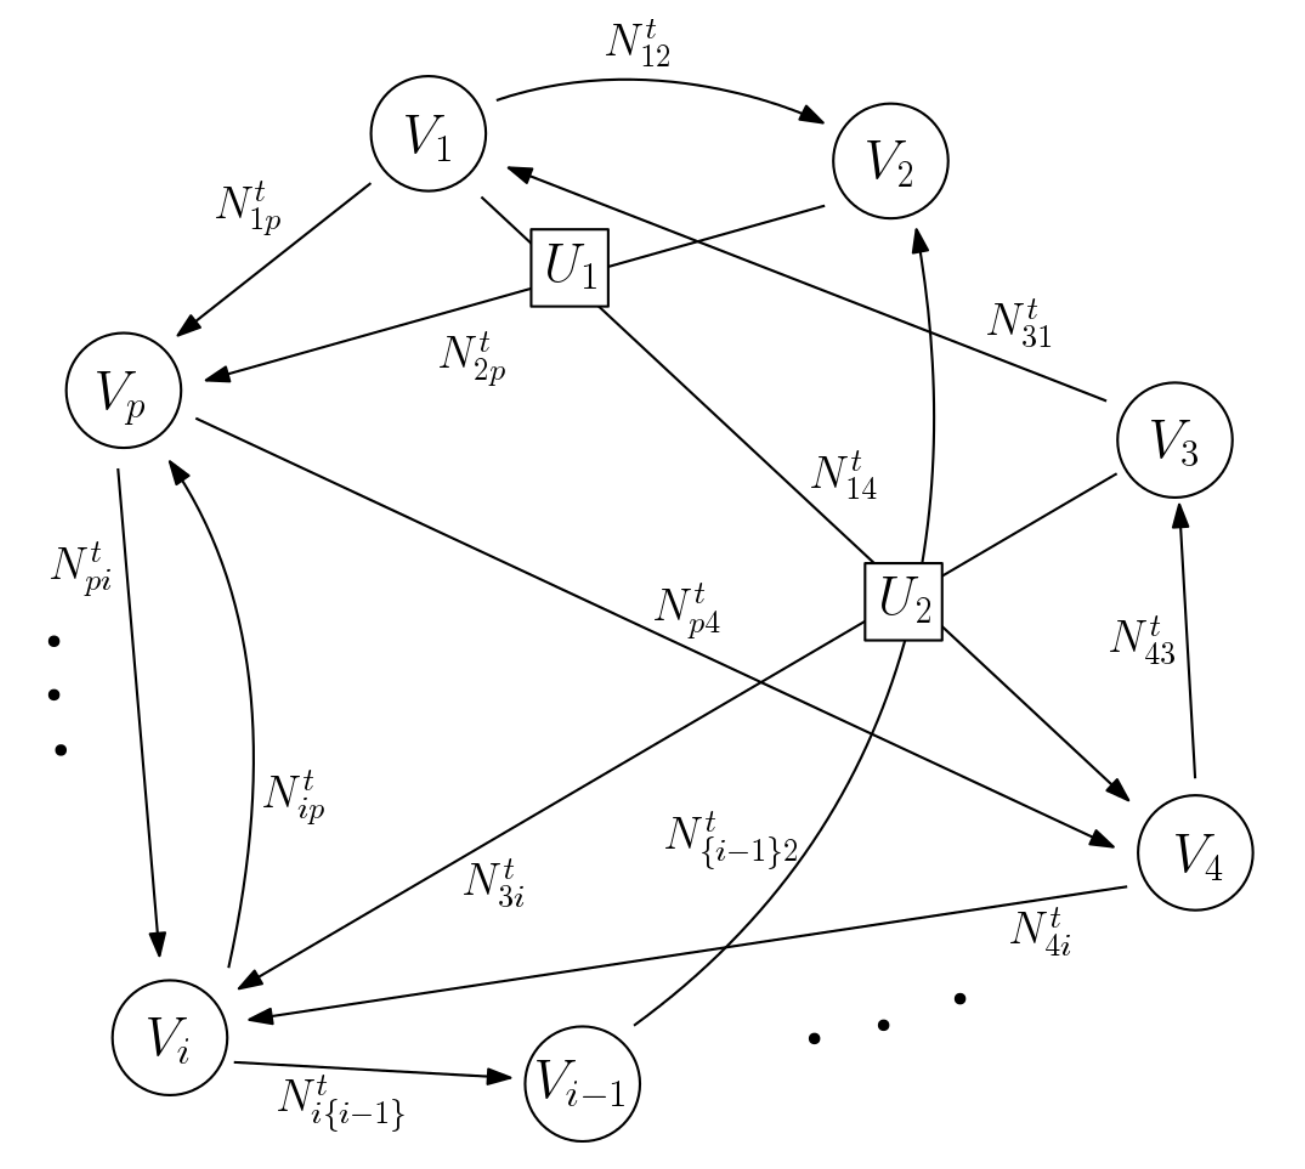
\includegraphics[width=0.35\textwidth]{Hou_Network}
	\caption{An array of facilities with shadow interactions proposed by Hou et al\cite{Hou_2016}}
	\label{fig:maximumlikelihood}
\end{figure}

The method proposed by Yilmaz et al. assumes 3 fuel enrichments and two shipment speeds for simplicity. Data are collected to establish a Poisson distribution of expected delivery time. The algorithm requires a training set of approximately 10 shipments before false positive rate is minimized \cite{Yilmaz_2016}. The benefit of this method is an increased response time without sacrificing as much accuracy as traditional cumulative sum methods. 

Scenarios without direct access to fuel orders require indirect observation by tracking the edges of a fuel cycle network. Increasing the number of known 'edges', or transportation routes, increase the algorithm speed with the only requirement of monitoring the intake and output of facilities rather than each shipment. Figure 1 demonstrates a partially observed network to which a hybrid minimum relative entropy model is applied. This technique results in a more lenient input compared to a maximum likelihood estimation that requires a majority of the network to be observed \cite{Hou_2016}.


This model requires approximately 150 observed time steps to attain similar false positive rates to a Poisson distribution, however, requires substantially less direct information. While the algorithm performs well over time in obscured fuel cycles, timely detection is required to prevent proliferation. The proposed algorithm seeks to adapt and include signatures and observables from pyroprocessing facilities, providing additional edges and information to a minimum relative entropy model. The algorithm should provide a compromise of the two detection methods for a new molten salt reprocessing cycle.

%%%%%%%%%%%%%%%%%%%%%%%%%%%%%%%%%%%%%%%%%%%%%%%%%%%%%%%%%%%%%%%%%%%%%%%%%%%%%%%%
\section{Conclusions}
This analysis demonstrates the variability in commercialized pyroprocessing facilities and potential signatures and observables that will aid diversion detection. \Cyclus also is outlined as tool in detecting shadow fuel cycles through its agent-based simulation and modular facilities, allowing for variations in plant design. Modeling and data collection of shadow fuel cycles will be performed in the \Cyclus environment after creation of a library specific to the unique needs of electrochemical refinement. Data from these simulations will be utilized in a minimum relative entropy model with additional signatures and observables to ideally reduce detection delay while maintaining high accuracy.

%%%%%%%%%%%%%%%%%%%%%%%%%%%%%%%%%%%%%%%%%%%%%%%%%%%%%%%%%%%%%%%%%%%%%%%%%%%%%%%%
\section{Acknowledgments}
This research was performed using funding received from the Consortium for Nonproliferation Enabling Capabilities under award number 1-483313-973000-191100.

%%%%%%%%%%%%%%%%%%%%%%%%%%%%%%%%%%%%%%%%%%%%%%%%%%%%%%%%%%%%%%%%%%%%%%%%%%%%%%%%
\bibliographystyle{ans}
\bibliography{bibliography}
\end{document}

